\section{Setup}
The experiment is conducted in a closed box containing the beam path and both measurement devices, a monochromator and a 
CCD spectrometer, attached. A sketch is displayed in figure~\ref{fig:setup}. 
Further devices for amplification of the monochromator's signal as well as sources for the 
laser current and the photomultiplier voltage are arranged on a rack. The beam path consists of a laser, a sample at which
the photons are scattered, optical lenses for focusing and one of the two spectrometers. Further included for various 
measurements are the following devices:
\begin{itemize}
    \item A $\lambda / 2$ plate inserted between laser and sample in order to turn the 
        polarization of the laser's light by $90^\circ$. The laser is polarized vertically, such that the radiation due to 
        Raman scattering would be virtually zero in direction of the beam path (at least in the case of symmetric
        vibrational modes).
    \item A notch filter in front of the CCD spectrometer used to reduce overflow due to the high intensity of the 
        Rayleigh peak compared to the Raman peaks. 
    \item A polarization filter with adjustable angle for a measurement of depolarization ratio of CCl$_4$. 
    \item A white light and a Hg-lamp for calibration and analysis of the spectrometers' parameters. 
\end{itemize}

\begin{figure}[htpb]
    \centering
    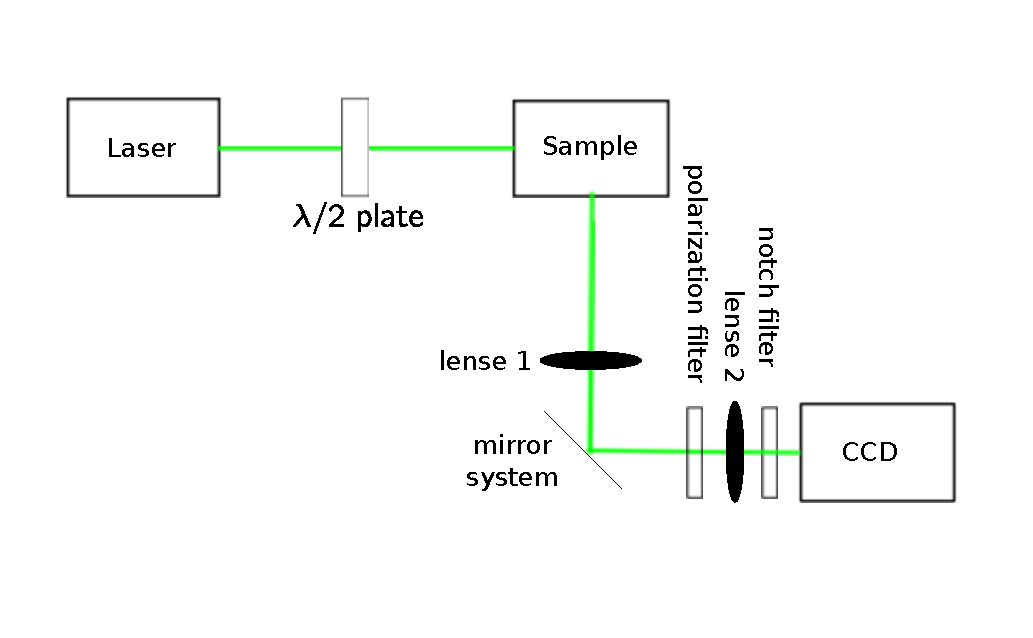
\includegraphics[width=0.8\linewidth]{figures/setup}
    \caption{
        Beam path of the Raman scattering experiment with CCD spectrometer. $\lambda / 2$ plate, polarization 
        filter and notch filter are not used in all cases.
        }
    \label{fig:setup}
\end{figure}

